% %%%%%%%%%%%%%%%%%%%%%%%%%%%%%%%%%%%%%%%%%%%%%%%%%%%%%%%%%%%%%%%%%%%%%%%%%%%%%
\chapter{Non-Autoregressive NMT}
\label{chap:nat}
% %%%%%%%%%%%%%%%%%%%%%%%%%%%%%%%%%%%%%%%%%%%%%%%%%%%%%%%%%%%%%%%%%%%%%%%%%%%%%

The efficiency of \ac{mt} models is often crucial in real-world applications.
Most commercial \ac{nmt} models are available through a cloud-based service,
such as Microsoft Translator\footnote{\url{https://microsoft.com/translator}}
or Google Translate\footnote{\url{https://translate.google.com}}. Scaling
cloud-based solutions for large user bases is simple but costly. But even with
a large pool of computational resources, it is worthwhile to implement
optimizations which decrease the model latency and improve the user experience.

% lokální modely maj tu výhodu, že to běží u mně, takže to jde pouyžít offline
% a taky se nemusím bát o svoje soukromý data. ale jsou pomalý.

Locally-deployed \ac{nmt} models provide a number of advantages over
cloud-based solutions. First, the service does not rely on internet
connection. Second, the data are not being sent to a 3rd party server, and
therefore it is suitable for translating private or confidential data.
However, without optimization, running state-of-the-art translation models
locally often requires specialized hardware, such as one or more GPU
cards. Otherwise, the time for translating a single sentence can easily reach
more than a second on a standard CPU.

Higher decoding speeds can be achieved by model optimization. In their 2019
submission to the \ac{wngt} shared task on efficiency,
\citet{kim-etal-2019-research} successfully employed knowledge distillation,
quantization, shortlisting \citep{jean2015using} and a simpler recurrent unit
design to bring the throughput of the translation model up to 3,600 words per
second on a CPU, for a modest drop in the BLEU score. Following this
submission, \citet{bogoychev-etal-2020-edinburghs} reported further
improvements with attention head pruning \citep{voita-etal-2019-analyzing}. The
work has been a part of the Bergamot research project, which aims to bring
offline translation models into a browser (\JH{cite}).

% vedle toho tu jsou neautoregresivní modely který se na to snaží jít jinak

\Ac{nar} models present an alternative approach to model optimization, using a
different architecture and decoding algorithm which has lower time complexity.
In \ac{nmt}, a non-autoregressive decoding algorithm does not access the
previously decoded outputs, imposing conditional independence on the output
token probability distributions. This assumption allows parallelization of the
decoding which can significantly reduce the latency of the translation
system. On the other hand, it also presents a challenge to the language model,
which usually leads to poorer translation quality.

The research presented in this thesis is focused on the usefulness of \ac{nar}
models for translation (\acs{nat}\glsunset{nat}) in the quest for faster
translation models. We first analyze the \ac{nat} models alone and assess the
necessary techniques needed to match the quality of \ac{ar} models.  Then, we
adapt the optimizations successfully used in \ac{ar} models for \ac{nar} models
and evaluate the additional speed gains.

\JH{Write chapter overview.}

% This chapter begins with an overview of the non-autoregressive methods (Section
% \ref{sec:nat-methods}). In Section \ref{sec:nat-ctc}, we introduce
% non-autoregressive \ac{nmt} with \ac{ctc}. \JH{rewrite following commented:}
% We present our experiments with \ac{ctc} in Section
% \ref{sec:ctc-experiments}. We summarize our contributions and outline the
% possible future efforts in Section \ref{sec:nat-future}.


% ------------------------------------------------------------------------------
\section{Related Work}
\label{sec:nat-methods}
% ------------------------------------------------------------------------------

This section presents the key concepts in non-autoregressive \ac{nmt}. We first
describe the principles that most of the related literature has in
common. Then, we provide a survey of notable approaches to \ac{nat}.

% ------------------------------------------------------------------------------
\paragraph{Conditional Independence.} The defining feature of a
non-autoregressive model is the conditional independence of the output
distributions across time steps. Recall Equation \ref{eq:output-distribution}
which defines the output distribution for autoregressive models:
%
\begin{equation*}
  p(y|x) = \prod_{t=1}^{T_y}p(y_t|y_{<t},x,\theta).
  \tag{\ref{eq:output-distribution}}
\end{equation*}
%
Unlike Equation \ref{eq:output-distribution}, \Ac{nat} models do not condition
the output token probabilities on the previously decoded outputs $y_{<t}$.  The
probability of an output sentence $y$ given an input sequence $x$ can then be
modeled as:
%
\begin{equation}
  p(y|x) = \prod_{t=1}^{T_y}p(y_t|x,\theta).
  \label{eq:nat-output-distribution}
\end{equation}

Although technically possible, making the outputs in \acs{rnn}-based models
conditionally independent does not reduce the decoding time because in
\acsp{rnn}, each state depends on the value of the preceding state. However, in
the Transformer model, the hidden states in one layer depend only on the states
from the previous layer. This allows for parallelization on the layer level.

Since the outputs are conditionally independent, the Transformer decoder cannot
work with the previously decoded outputs. In the following paragraphs, we
discuss the necessary alterations to the Transformer architecture.  First, the
decoder needs to know the sentence length. Second, we need to supply the
decoder inputs. Third, the causal mask in the decoder self-attention is now
unnecessary.

% ------------------------------------------------------------------------------
\paragraph{Target Length Estimation.} In a standard NMT model such as the
Transformer or an \acs{rnn}-based model with attention, the length of the
output sentence is modeled implicitly by using the special end-of-sentence
(\eos{}) token. Equations \ref{eq:output-distribution} and
\ref{eq:nat-output-distribution} work with the sentence length implicitly,
assuming that the last token $y_{T_y}$ is the \eos{} token and that \eos{} does
not appear among the previous tokens $y_{<T_y}$.

The probability distribution in Equation \ref{eq:nat-output-distribution} can
be factorized to express the estimation of the target sentence length
explicitly, leaving out the \eos{} symbol from the mathematical model:
\begin{equation}
  p(y|x) = p_L(T_y|x, \theta) \cdot \prod_{t=1}^{T_y}p(y_t|x,\theta).
  \label{eq:explicit-length}
\end{equation}


% When using Equation \ref{eq:output-distribution} to model probability
% distribution over the set of all possible sentences, the probabilities assigned
% to longer sentences are considerably lower than the probabilities of sentences
% which are short. This follows from the multiplication of probabilities, which
% are numbers between zero and one. \JH{další věc je že je ten search space
%   exponenciálně roste -- This follows from the fact that the search space
%   (i.e. the number of all possible sentences of length $T_y$) grows
%   exponentially with $T_y$.}  \JH{odkazat spis na argmax nez na output
%   distribution.} To diminish the negative influence of this property,
% \citet{wu2016google} introduce length normalization to the beam search algorithm
% (\JH{odkazat na eq. v intro do MT}). The normalization acts as a prior imposed
% on the target sentence length distribution.

% It is, however, possible to estimate the target length explicitly.
% \JH{...}

\JH{mention these:}
\citep{ghazvininejad2019mask} \citep{mansimov2019generalized}

% ------------------------------------------------------------------------------
\paragraph{Multimodality Problem.} In one of the first applications of a
non-autoregressive model to \ac{nmt}, \citet{gu2017nonautoregressive} describe
the \emph{multimodality problem} which arise when the outputs are conditionally
independent.

When estimating the probability of a word on a given position, there may be
multiple words which get a high probability. These words are the so called
\emph{modes} of the distribution. In autoregressive models, once a word gets
selected, other modes are ignored in the following time steps. However, a
non-autoregressive model does not base the decisions on the preceding ones, so
when multiple positions have multiple modes, the model has no way of knowing
which modes have been selected on other positions.

% This issue is illustrated in Figure \ref{fig:multimodality-problem}.
% \begin{figure}
%   \centering
%   \begin{minipage}{\textwidth}
%     source: thank you

%     \begin{center}
%     \begin{tabular}{cccc}
%       \toprule
%       $y_1$ & $p(y_1|x)$ & $y_2$ & $p(y_2|x)$ \\
%       \midrule
%       vielen & 0.4 & dank & 0.4 \\
%       danke  & 0.3 & schön & 0.3 \\
%       \vdots & & \vdots & & \\
%       \bottomrule
%     \end{tabular}
%     \end{center}

%   \end{minipage}
%   \caption{Illustration of the multimodality problem.}
%   \label{fig:multimodality-problem}
% \end{figure}

A well-known example of the multimodality problem is the translation of the
sentence ``thank you'' into German, which has two equally likely translations:
``vielen dank'' and ``danke schön.'' In this case, the pair of German tokens
``danke'' and ``vielen'' create the two modes on the first position, and the
tokens ``dank'' and ``schön'' are modes on the second position. If an
autoregressive model chooses to generate ``danke'' on the first position, the
token ``dank'' on the second position will no longer be likely. However, when a
non-autoregressive model assigns high probabilities to the correct
translations, it also has to assign high probabilities to the other (incorrect)
two combinations, ``danke dank'' and ``vielen schön''.

% ------------------------------------------------------------------------------
\paragraph{\Ac{nat} with Fertility Model.} Non-autoregressive Transformer
decoder does not receive the previously decoded tokens on the input. A solution
proposed by \citet{gu2017nonautoregressive} is to use a simple fertility model,
which also serves as the explicit target length estimator.

Compared to the autoregressive Transformer model, the model has the following
modifications. First, the inputs to the decoder are made up of the sequence of
encoder inputs, either uniformly stretched to the predicted target sentence
length, or copied using a fertility model. Second, the decoder self-attention
does not use the causal mask since all states can now attend to all other
states in both directions. Third, \emph{positional attention} is added to every
decoder layer where the positional encoding is used as queries and keys, and
the decoder states as values.

In \citet{gu2017nonautoregressive}, the multimodal problem is addressed by
introducing a latent fertility variables $f_1, \ldots, f_{T_x}$ sampled from a
prior distribution. Each $f_i \in \mathbb{N}_0$ denotes the number of times to
copy $x_i$ to the decoder input. The output probability is then conditioned on
the value of the latent variable.
% \begin{equation}
%   p(y|x) = p_L(T_y|x, \theta) \cdot \prod_{t=1}^{T_y}p(y_t|x, z, \theta).
% \end{equation}

The training is done by combining two loss functions -- translation loss and
fertility loss:
\begin{align}
  \mathcal{L}(\theta)  & = \log p(y|x, \theta) \\
                       & = log \sum_{F \in \mathcal{F}} p(F| x, \theta ) p(y | x, F, \theta) \\
                       & \geq \mathbb{E}_{\bar{F} \sim q}
                         \left(
                         \sum_{t=1}^{T_y} \log p(y_t | x, \bar{F}, \theta)
                         + \sum_{t=1}^{T_x} \log p(f_t | x, \theta)
                         \right)
                         + \mathcal{H}(q)
\end{align}
%
where \JH{... describe the equation, or comment it out. Also, what is $\mathcal{H}$?}
%
The fertility model depends on an external module and is not trained end to
end. The authors fine-tune the trained model using reinforcement learning
\citep{williams1992simple}.

During decoding, the marginalizing over all possible fertility values is
intractable. Therefore, the authors experiment with three approximation methods
-- argmax and average decoding, and \ac{npd}.

% ------------------------------------------------------------------------------
\paragraph{Knowledge Distillation.} To tackle the multimodality problem from
another angle, \citet{gu2017nonautoregressive} propose to use sequence-level
knowledge distillation to create artificial training data
\citep{kim-rush-2016-sequence}. The main idea is that outputs of a teacher
model will have a simpler structure than natural language, limiting the number
of the distribution modes.

According to an ablation study published by \citet{gu-kong-2021-fully}, using
knowledge distillation is a crucial element in training non-autoregressive
translation models, regardless the actual method used.

% ------------------------------------------------------------------------------
\paragraph{Iterative Refinement.} Another attempt to introduce latent variables
in a non-autoregressive model was proposed by
\citet{lee-etal-2018-deterministic}.  Instead of modeling fertility, the
authors introduce $L$ discrete sequential latent variables interpreted as
stages of refinement:
%
\begin{align}
  \begin{split}
    p(y|x) & = \sum_{y^L}
      \left( \prod_{t=1}^{T_y} p(y_t|y^L, x) \right) p(y^L|x) \\
    p(y^L|x) & = \sum_{y^{L-1}}
      \left( \prod_{t=1}^{T_y} p(y_t^L | y^{L-1}, x) \right)
      p(y^{L-1}|x) \\
    \vdots \\
    p(y^0|x) & = \prod_{t=1}^{T_y} p(y_t^0|x)
  \end{split}
\end{align}
%
Each summation in the equations above is computed over the whole space of
possible sequences, and thus, it is intractable for the probablility $p(y|x)$
to be caluculated exactly. To overcome this problem, the authors approximate
the sums with only the element corresponding to the sequence with the largest
probability, $\hat{y}_t = \argmax_{y_t}p(y_t|x)$.\footnote{Note that in
  non-autoregressive model where the probability does not depend on previously
  decoded outputs $y_{<t}$, getting the most probable tokens will also yield
  the most probable sequence.}  Putting it together with the equations above
and moving to the logarithmic domain, we get:
\begin{align}
  \begin{split}
    \log p(y|x) \geq
    & \sum_{t=1}^{T_y} \log p(y_t| \hat{y}^L, x) + \\
    & + \sum_{t=1}^{T_y} \log p(\hat{y}_t^{L}| \hat{y}^{L-1}, x) + \ldots \\
    & + \sum_{t=1}^{T_y} \log p(\hat{y}_t^0 | x). \label{eq:refinement-lowerbound}
    % = & \sum_{l=0}^{L} \sum_{t=1}^{T_Y} \log p(\hat{y}_t^{l+1} | \hat{Y}^l, X)
  \end{split}
\end{align}
%where $Y^0 = X$ and $\hat{y}_t^{L+1} = y_t$.

The initial sequence $\hat{y}_t^0$ is set to $x_{t'}$ where
$t' = (T_x / T_y) \cdot t$, i.e. the source sentence is either squished or
stretched by copying or omitting some of the source words in order to fit the
target sentence length. During training, the length of the reference sentence
is known. During decoding, the authors use a separate model $p(T_y|x)$ for
target length prediction. All probability distributions in the above equations
are modeled with neural networks with shared parameters. In this way, the
number of intermediate refinement steps remains flexible during the decoding.

The latent variable model is trained by minimizing the log-likelihood of the
eference sentence $y^*$ in each of the refinement steps:
\begin{equation}
  \mathcal{L}_{\text{LVM}}(\theta) = - \sum_{l=1}^{L+1} \left(
    \sum_{t=1}^{T_{y^*}} \log p(y_t^* | \hat{y}^{l-1}, x, \theta)
  \right) \label{eq:refinement-lvm-loss}
\end{equation}

In their iterative approach, \citet{lee-etal-2018-deterministic} also discuss
the training of the refinement process from a denoising perspective. Formally,
they introduce an additional denoising autoencoder loss to the model:
%
\begin{equation}
  \mathcal{L}_{\text{DAE}}(\theta) = - \sum_{t=1}^{T_y} \log p(y_t^* | \bar{y}, x, \theta)
\end{equation}
where $\bar{y}$ is a corrupted version of the reference translation $y^*$. The
corruption process is performed on each token with a probability $\beta$. Each
corrupted token is either replaced with a random word from the vocabulary,
copied to its neighbor, or swapped with the neighbor.

During training, the two loss functions are stochastically mixed using a
hyperparameter $\alpha$, sampled from a Bernoulli distribution.


% ------------------------------------------------------------------------------
\paragraph{Aligned Cross Entropy for \ac{nat}} One problem with using
cross-entropy objective for training \ac{nat} models is that it heavily
penalizes misaligned target words. If a correct word is generated at an
incorrect position in the target sentence, the loss is the same as when the
model generates a completely unrelated word. In autoregressive models, this
problem is avoided with teacher forcing -- the model is provided with the
preceding words from the reference sentence. Without teacher forcing, the
alignment between the predicted distributions and the positions in the
reference sentence is too rigid. For example, consider the reference sentence
``Thank you for your cooperation.'' In a non-autoregressive model, another
translation ``Thanks for your cooperation'' receives the same training signal
as a completely wrong translation. The difference is that on the second
position, the autoregressive model knows that ``Thank'' was expected on the
first position, so the next word ``for'' does not receive high probability.
One way to address this problem is to consider the alignment as a latent
variable.

\Acl{axe} \glsunset{axe} (\acs{axe}; \citealp{ghazvininejad2020aligned}) is an
objective function that takes this problem into account. It uses a dynamic
programming algorithm to find the alignment with the minimum cross-entropy
loss. In the example from the previous paragraph, the alignment with the lowest
cross-entropy is the one that aligns the positions 3--5 from the label sequence
(representing the suffix ``for your cooperation'') to output positions 2--4 in
the output. Either of the first two positions in the label sequence can be
aligned to the first position in the output sequence, while the other label
position remains unaligned.

It is possible for the alignment to either skip a target position (as in the
example above), or keep an unaligned position in the prediction sequence. In
case of skipping the predictions, an empty token is aligned with the skipped
position (so that $-\log p(y_t = \epsilon)$ is added to the loss). In case of
skipping a target position, the negative log probability of the skipped target
word is added to the loss, weighted by a hyperparameter $\delta$ which controls
the cost of the skip-target operation.

Formally, ... \JH{doplnit}

In our experiments, we use the \ac{ctc} loss, which is similar to this
approach. Instead of considering the alignment that yields the minimum
cross-entropy loss, the \ac{ctc} algorithm computes the sum of all the possible
alignments. Unlike \ac{axe}, we only consider skipping the predictions, while
not allowing to skip the target positions. We present the \ac{ctc}-based method
in detail in Chapter \ref{chap:nar-nmt-ctc}.

\JH{relate the axe approach to bag-of-ngrams who also deal with misalignment}
\paragraph{\JH{Batch of ngrams.}} \citet{shao2020minimizing} also address the
misalignment issue. Instead of finding an appropriate alignment, they introduce
a new bag-of-ngrams objective, which minimizes the difference between the
\ac{nat} model output and the target sentence. \JH{tell me more!}



% ------------------------------------------------------------------------------
\paragraph{Iterative Decoding from Masked Language Models.} Recently,
pre-trained \acp{mlm} such as BERT \citep{devlin-etal-2019-bert} have attracted
attention from the translation research
community. \citet{ghazvininejad-etal-2019-mask} introduce \acp{cmlm}, an
extension to \acp{xlm} for multilingual applications, including \ac{mt}
\citep{conneau-lample-2019-cross}.

Unlike conventional language models that estimate the probability of a word
given the preceding words, \acp{mlm} are trained to predict words on masked
positions inside a sequence. Instead of working with a monolingual sequence,
\acp{xlm} extend this idea to a pair of sequences in two (or more) languages.
To facilitate for alignment modeling and language identification, \ac{xlm}
architectures include a language embedding and reset the positional encodings
for each sentence. See Figure \ref{fig:mlm-xlm-example} for an illustration of
differences between \acp{mlm} and \acp{xlm}.

\begin{figure}
  \centering

  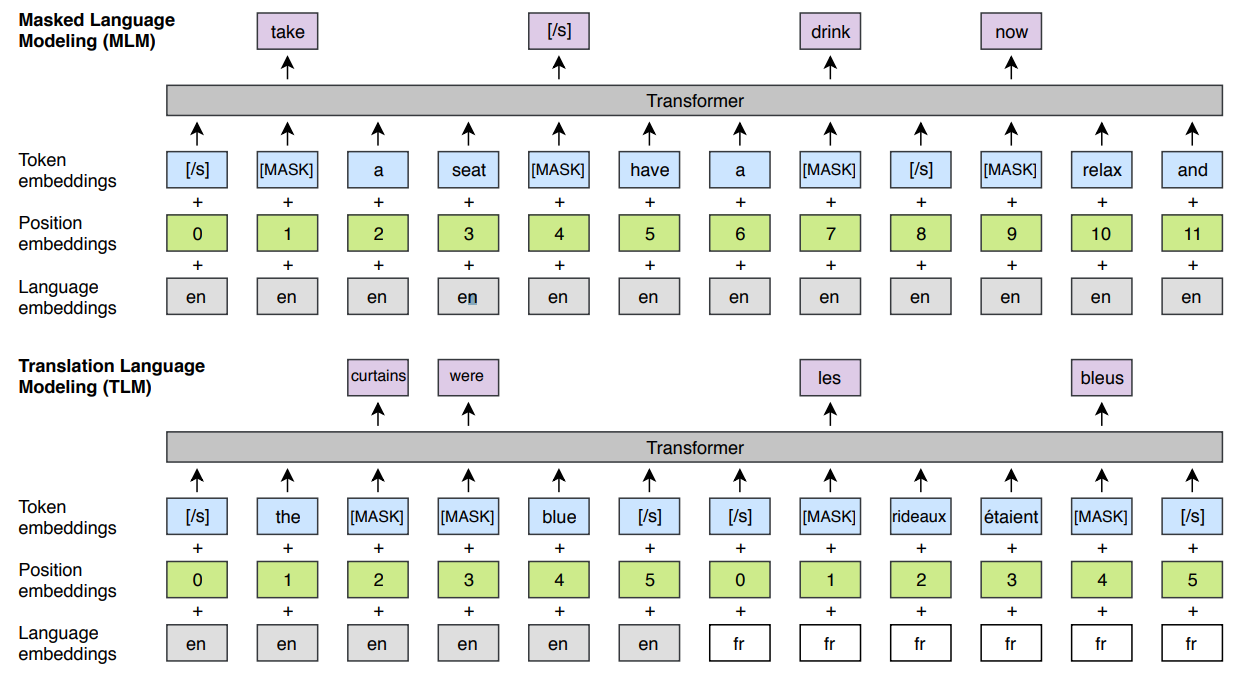
\includegraphics[width=\textwidth]{img/mlm-xlm.png}

  \caption{A comparison of masked language model and translation
    (cross-lingual) language model architectures. We use the image of
    \citet{conneau-lample-2019-cross}.}%
  \label{fig:mlm-xlm-example}
\end{figure}





% ------------------------------------------------------------------------------

\paragraph{Blockwise Parallel Decoding for Deep Autoregressive Models.}
\citet{stern2018blockwise} propose a semi-autoregressive approach where chunks
of the target sentence are generated in parallel.
%
They start with a greedy decoding from an autoregressive model, $p_1$, and
introduce additional ``look-ahead'' models $p_2, \ldots p_k$. In time step $t$,
each model $p_i$ predicts the $(t + i)$-th word in the target sequence given the
same prefix of $t$ previously decoded words.

The decoding process has three stages. First, the block of predictions using the
models $p_1, \ldots, p_k$ is computed. Second, model $p_1$ is used to verify the
$(k-1)$ candidates (which is done in parallel in the Transformer model) and
finds the largest $\hat{k}$ such that decoded words from models $p_i$,
$1 \leq i \leq \hat{k}$ are all considered best by $p_1$. Third, the accepted
$\hat{k}$ words are generated and the decoding process jumps to time step
$t + \hat{k}$.






% ------------------------------------------------------------------------------

\JH{add semiautroegressive paper from emnlp 2018}

\begin{itemize}
%\item iNat \citep{lee2018deterministic} -- iterative refinement
%\item Blockwise \citep{stern2018blockwise}
\item InsT \citep{stern2019insertion} -- insertion transformer
%\item CMLM \citep{ghazvininejad2019mask} -- conditional masked language models
\item LevT \citep{gu2019levenshtein} -- Levenshtein transformer
\item KERMIT \citep{chan2019kermit} -- Kermit (arxiv)
\item LaNMT \citep{shu2020latent} -- latent-variable NAR NMT with deterministic inference using a delta posterior
\item SMART \citep{ghazvininejad2020semiautoregressive} -- semi-autoregressive training improves mask-predict decoding
\item DisCO \citep{kasai2020nonautoregressive} -- NAR NMT with disentangled context transformer
\item Imputer \citep{saharia2020nonautoregressive} -- NAR NMT with latent alignments
\end{itemize}

Fully NAT:


% ------------------------------------------------------------------------------

\paragraph{Latent Transformer \citep{kaiser2018fast}.} Latent transformer (fast
decoding in seq. models using discrete latent vars) Use latent variables to make
decoding parallelizable. Auto-encode targets to latent variables which are
predicted autoregressively, then decode from these latent variables in
parallel. Mostly use one eigth of the original sentence length.

Unlike perhaps more common autoencoders, this autoencoder uses discrete latent
variables.  The discretization is studied and decomposed vector quantization
(DVQ) or latent semantic hashing is proposed as best-performing. Generally,
$enc(y) \in \mathbb{R}^D$, where $D$ is latent space dimension. $[K]$ is the
discrete latent space alphabet. $enc(y)$ is discretized to two latent variables
$z_d(y) \in K$ as the latent representation and $z_q(y)$ as input to the
decoder. $\tau_m(i)$ is binary representation of $i$ using $m$ bits.

\textbf{Gumbel softmax} -- produce logits $l = W \text{enc}(y)$,
$W \in \mathbb{R}^{K \times D}$, then take argmax to get $z_d(y)$. Decoder input
$z_q(y)$ is embedding of $z_d(y)$. To make this argmax differentiable, during
training, Gumbel-Softmax trick is used: $g_1, \ldots, g_K$ are sampled from
Gumbel distribution, $g_i \sim -\log(-\log u)$, where $u \sim U(0,1)$, and:
\begin{equation}
  w_i= \frac{\exp((l_i + g_i) / \tau) }{\sum_i exp((l_i + g_i)/\tau)}
\end{equation}
to get $w \in \mathbb{R}^K$, and use $z_q(y) = w \times E$. Gumbel-softmax is
simply used as differentiable sampling from intermediate logits.

\textbf{Improved semantic hashing} -- use rounding bottleneck after squashing
encoder state $z_e(y)$ using saturating sigmoid:
\begin{equation}
  \sigma'(x) = \max(0, \min(1, 1.2 \sigma(x) - 0.1))
\end{equation}
During training, gaussian noise is added before the saturating sigmoid to
encoder states $z_e(y)$: $f_e(y) = \sigma'(z_e(y) + \eta ~ N(0,1)^D)$. Discrete
latent representation, binary vector $g_e(y)$ is constructed by rounding
$f_e(y)$ to zeros and ones. $z_d(y)$ is computed as $\tau^{-1}_{log_K}(g(y))$
(that is, by conversion of $g_e(y)$ from binary to decimal with base $K$). The
input $z_q(y) = e^1_{h_e(y)} + e^2_{1-h_e(y)}$ where $h_e(y)$ is either $f_e$ or
$g_e$ during training, but only $g_e$ during inference.

\textbf{Vector quantizated variational autoencoder (VQ-VAE)} --
$enc(y)\in\mathbb{R}$ mapped on embeddeding $e\in\mathbb{R}^{K\times D}$ as
nearest-neighbor lookup. $z_q(y) = e_k$, whereoq
$k = argmin_{j\in[K]} || enc(y) - e_j ||_2$, latent $z_d(y)$ being $k$. This is
trained with reconstruction loss, and $enc(y)$ being drawn to fixed values of
$z_q(y)$. They also keep moving averages of the embeddings and the counts,
EM-like.

\textbf{DVQ} -- the former has an issue with a few indices receiving the most signal
during training. Proposed two solutions: sliced VQ and projected VQ. In sliced,
idea is to slice $enc(y)$ to smaller vectors and do the nearest neighbor using
the sslices, reconstructing $z_q(y)$ from the results. In projected, instead of
slicing, the vector is projected multiple times to subspace.

The model has three components: autoencoder $ae(y, x)$ which maps $y$ to shorter
latent sequence $l$, latent prediction model $lp(x)$ which produces $l$ out of
$x$, and decoder $ad(l, x)$ which non-autoregressively produces $y$ out of $l$
and $x$. They use two losses with equal weights: recunstruction loss computed
from $ad(ae(y,x),x)$ and latent prediction loss comparing $ae(y,x)$ and $lp(x)$.
The latent predictor is a transformer, the autoencoder is stack of convolutions
with residual connections, and the decoder consists of up-convolutions.

Results measured on WMT'14 EN-DE. Baseline 27.3 BLEU, they achieve 22.5 with
rescoring. p-DVQ and s-DVQ as well as improved semhash are comparable, semhash
seems faster. Latency in the order of 100 ms, 7-8 ms per sentence with batch
size of 64.



\subsection{Auxiliary Objective Methods}


% ------------------------------------------------------------------------------
\paragraph{\Ac{nat} with auxiliary regularization.}
\citet{wang-etal-2019-nonautoregressive} use regularization terms to penalize
similarity of hidden states corresponding to dissimilar words(which battles
repeated translations), and to express a reconstruction loss using an external
translation model (in order to battle incomplete translation
problem). \JH{NAT-REG}

% ------------------------------------------------------------------------------
\paragraph{Hint-NAT.} \citet{li-etal-2019-hint} propose to regularize the
training of the student \ac{nat} model using two types of signals (hints) from
the \ac{ar} teacher. First, to bring the values of the decoder hidden states
closer together the authors consider tying the teacher and student states with
$L_1$ or $L_2$ distance, but argue that this straightforward approach
destabilizes the student training process and fails. Instead, they use a weaker
signal from the teacher model and define an auxiliary loss based on the cosine
distances within the decoder hidden states. Second, they use the information
from the teacher model cross-attention to guide the alignment learning in the
student model. Again, this information is incorporated into the training as an
auxiliary loss, based on the KL divergence between the teacher and student
attention distributions.

\JH{Add equations for the auxiliary losses? Ich dont think so..} \JH{Unify
  losses, it's either $J$ or $\mathcal{L}$}



% -----------------------------------------------------------------------------
\paragraph{ReorderNAT.} \citet{ran-etal-2021-guiding} \JH{this is not an
  auxiliary objective}


% -----------------------------------------------------------------------------
\begin{itemize}
\item DCRF \citep{sun2019fast} -- fast structured decoding for sequence models
\item Flowseq \citep{ma2019flowseq} -- NAR conditional sequence generator with generative flow
\item EM+ODD \citep{sun2020em} -- an em approach to NAR conditional seq generation
\item GLAT \citep{qian2020glancing} -- glancing transformer for NAR NMT
\item Imputer \citep{saharia2020nonautoregressive} -- imputer (again)
\item \citep{huang-etal-2021-nonautoregressive} -- layer-wise prediction and deep supervision (is it semi or not?)
\end{itemize}

\section{Discussion}

\JH{Here should be a section on the limitations of the presented papers}

\JH{Many papers claim that reordering is an issue. While this might be true,
  the culprit is the multimodality problem, as the reordering can be modeled
  within the self-attentive layers. Also, the papers that propose methods to
  model the reordering better, evaluate their method only on the end task
  (translation) and do not assess the actual reordering ability. }

\JH{We should also have a table with autoregressive baselines reported by each
  study, and get some details on that.}


\begin{table}
  \centering

  \begin{tabular}{ll}
    \toprule

    \midrule

    \bottomrule
  \end{tabular}

  \caption{An overview of the \ac{nat} models in the literature.}%
  \label{tab:related-models}
\end{table}

%%% Local Variables:
%%% mode: latex
%%% TeX-master: "thesis"
%%% End:
